\documentclass[crop,class=article]{standalone}
%----------------------------Preamble-------------------------------%
\usepackage[dvipsnames]{xcolor}         % Color names.
\usepackage{tikz}                       % Drawing/graphing tools.
\usetikzlibrary{arrows.meta}            % Latex and Stealth arrows.
%--------------------------Main Document----------------------------%
\begin{document}
    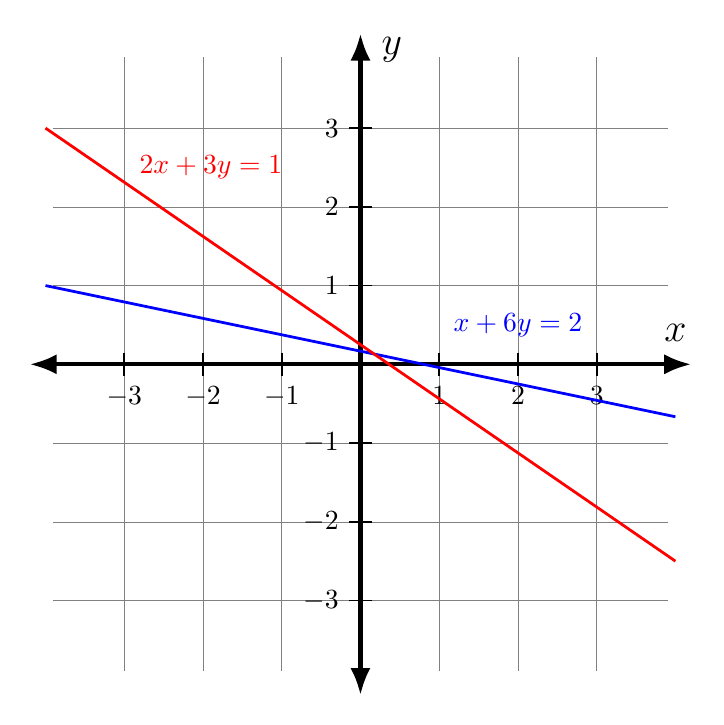
\begin{tikzpicture}[>=latex, line width=1pt]
        \draw[style=help lines] (-3.9, -3.9) grid (3.9, 3.9);
        \begin{scope}[line width=1.5pt, >=Latex, font=\Large]
            \draw[<->] (-4.2, 0) to (4.2, 0);
            \draw[<->] (0, -4.2) to (0, 4.2);
            \node at (4, 0.4) {$x$};
            \node at (0.4, 4) {$y$};
        \end{scope}
        \foreach\x in {-3, -2, -1, 1, 2, 3}
            \draw[shift={(\x,0)}, semithick]
                (0, 0.15) -- (0, -0.15) node[below] {$\x$};
        \foreach\y in {-3, -2, -1, 1, 2, 3}
            \draw[shift={(0, \y)}, semithick]
                (0.15, 0) -- (-0.15, 0) node[left] {$\y$};
        \draw[draw=blue] (-4,1) to (4,-0.666);
        \draw[draw=red] (-4,3) to (4,-2.5);
        \node at (-1.9, 2.5) {$\color{red}2x+3y=1$};
        \node at (2, 0.5) {$\color{blue}x+6y=2$};
    \end{tikzpicture}
\end{document}